% !TeX TS-program = txs:///latexmk | txs:///view-log | txs:///view-pdf | txs:///convert
\documentclass{article}
\usepackage{tikzducks}

\usepackage{geometry}

\begin{document}


\begin{tikzpicture}
	\duck
\end{tikzpicture}
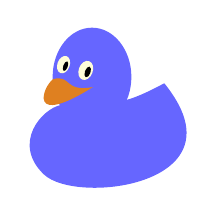
\begin{tikzpicture}
	\duck[body=blue!60!white]
\end{tikzpicture}

\begin{tikzpicture}
	\duck[grumpy, bill=cyan]
\end{tikzpicture}

\begin{tikzpicture}
	\duck[longhair=teal]
\end{tikzpicture}


\begin{tikzpicture}
	\duck[shorthair]
\end{tikzpicture}

\begin{tikzpicture}
	\duck[crazyhair=green!50!blue]
\end{tikzpicture}

\begin{tikzpicture}
	\duck[recedinghair=gray]
\end{tikzpicture}

\begin{tikzpicture}
	\duck[eyebrow]
\end{tikzpicture}


\begin{tikzpicture}
	\duck[tshirt=violet]
\end{tikzpicture}
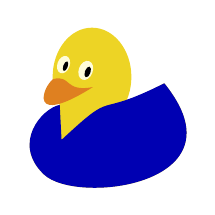
\begin{tikzpicture}
	\duck[jacket=blue!70!black]
\end{tikzpicture}
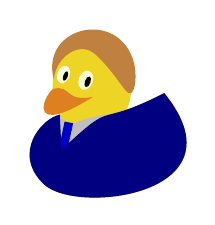
\begin{tikzpicture}
	\duck[tshirt=lightgray, 
			jacket=blue!50!black, 
			tie=blue!80!black, 
			shorthair]
\end{tikzpicture}
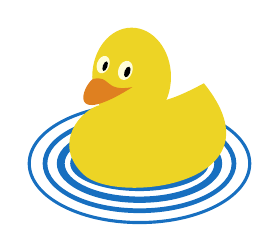
\begin{tikzpicture}
	\duck[water=cyan!50!blue]
\end{tikzpicture}


\begin{tikzpicture}
	\duck[alien=green!50!brown]
\end{tikzpicture}

\begin{tikzpicture}
	\duck[hat=red!50!black]
\end{tikzpicture}
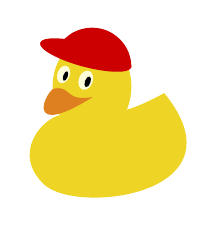
\begin{tikzpicture}
	\duck[cap=red!80!black]
\end{tikzpicture}

\begin{tikzpicture}
	\duck[body=pink,
		unicorn=magenta!60!violet,
		longhair=magenta!60!violet]
\end{tikzpicture}


\begin{tikzpicture}
	\duck[glasses=red!50!black]
\end{tikzpicture}

\begin{tikzpicture}
	\duck[sunglasses=blue]
\end{tikzpicture}

\begin{tikzpicture}
\duck[book=\scalebox{0.6}{$\pi$}, bookcolour=blue!50!black]
\end{tikzpicture}

\begin{tikzpicture}
	\duck[magichat,
				magicwand]
\end{tikzpicture}


\begin{tikzpicture}
	\duck[icecream]
\end{tikzpicture}
\begin{tikzpicture}
\duck
\path[preaction={fill, red!50!black},pattern=fivepointed stars, pattern color=yellow]  
\duckpathlonghair;
\end{tikzpicture}
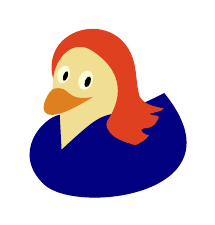
\begin{tikzpicture}
	\duck[body=yellow!50!brown!50!white, 
		longhair=red!50!brown, 
		jacket=blue!50!black]
\end{tikzpicture}

\begin{tikzpicture}
	\duck[cap,cricket]
\end{tikzpicture}


\begin{tikzpicture}
\definecolor{brazilgreen}{RGB}{0,155,58}
\definecolor{brazilyellow}{RGB}{254,223,0}
\definecolor{brazilblue}{RGB}{0,39,118}
	\duck[body=brazilyellow,
				shorthair=brazilgreen]
	\path[preaction={fill, brazilblue},pattern=fivepointed stars, pattern color=white] 
	\duckpathjacket;
\end{tikzpicture}

\begin{tikzpicture}
	\duck[grumpy, body=yellow!50!brown!50!white, tshirt=white, jacket=black, tie=black, hat=black, sunglasses=black]
\end{tikzpicture}

\begin{tikzpicture}
	\duck[body=yellow!50!brown!40!white,
		crazyhair=gray!50!white,
		eyebrow,
		glasses=brown!70!black,
		book=\scalebox{0.2}{$E=mc^2$},
		bookcolour=red!20!brown]
\end{tikzpicture}

\begin{tikzpicture}
	\duck[body=yellow!50!red!20!white,
		recedinghair=gray!50!white,
		eyebrow,
		tshirt=white!93!black,
		jacket=red!50!black,
		glasses=brown!70!lightgray,
		book=\scalebox{0.5}{\TeX},
		bookcolour=black!20!brown]
\end{tikzpicture}

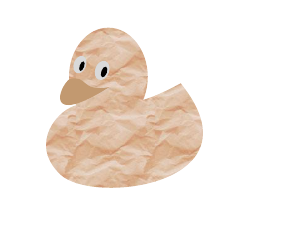
\begin{tikzpicture}[path image/.style={path picture={\foreach \j in {0,...,2}{\node at (0,\j) {\foreach \i in {1,...,5}{\includegraphics[height=1cm]{#1}}};}}}]
\path [path image=crinklepaper] 
	(0.90,1.50) ellipse (0.50 and 0.625);
\path [path image=crinklepaper] \duckpathbody;
\fill [orange!40!gray!80!white]  \duckpathbill;
\fill[white!70!gray, rotate=-20]
	(0.23,1.7675) ellipse (0.0893 and 0.125);
\fill[black, rotate=-20]
	(0.26,1.7575) ellipse (0.0357 and 0.0714);
\fill[white!70!gray, rotate=-20]
	(-0.06,1.74) ellipse (0.0786 and 0.1143);
\fill[black, rotate=-20]
	(-0.03,1.73) ellipse (0.0286 and 0.0643);
\end{tikzpicture}

\end{document}

